\documentclass[cn, hazy, blue, normal, 12pt]{elegantnote}

\title{高级计算机系统结构笔记}
\author{Mobyw}
\institute{Created by Elegant\LaTeX{}}
\version{1.0}
\date{\zhtoday}

\usepackage{tikz}
\usepackage{pgfplots}
\usepackage{bookmark}
\usepackage{multirow}
\usepackage{tabularx}
\usepackage{graphicx}

\pgfplotsset{compat=1.18}

\begin{document}

\maketitle

\section{量化设计与分析基础}

\subsection{计算机的分类}

\textbf{Flynn's 分类:基于指令流和数据流数量的计算机结构分类}

\begin{itemize}
    \item SISD: 串行计算机
          \begin{itemize}
              \item 任一时钟周期只有单个指令流在 CPU 执行,单个数据流用作输入
              \item 确定执行: 给定输入条件下多次运行的执行流程和结果一致
          \end{itemize}
    \item SIMD: 处理数据级并行
          \begin{itemize}
              \item 任一时钟周期所有处理单元执行相同指令
              \item 每个处理单元能对不同数据进行操作
          \end{itemize}
    \item MISD: 处理数据级并行
          \begin{itemize}
              \item 单个数据流进入多个处理单元
              \item 每个处理单元的指令流对数据独立进行操作
          \end{itemize}
    \item MIMD: 任务级并行
          \begin{itemize}
              \item 每个处理器可以执行不同的指令流,也可以对不同数据流进行操作
          \end{itemize}
\end{itemize}

Flynn 分类模型是抽象和粗略的,现代的不少并行处理器是 SISD、SIMD 和 MIMD 的混合类型.

\textbf{市场分类}

\begin{itemize}
    \item 个人移动设备
    \item 桌面计算机
          \begin{itemize}
              \item 个人计算机
              \item 工作站
          \end{itemize}
    \item 服务器:多处理器结构
          \begin{itemize}
              \item 可靠性
              \item 可扩展性
              \item 吞吐量
          \end{itemize}
    \item 集群/仓库级计算机
    \item 嵌入式计算机:实时性能
          \begin{itemize}
              \item 实时性能
              \item 软件固化
          \end{itemize}
\end{itemize}

\begin{figure}
    \centering
    \begin{tabular}{cc}
        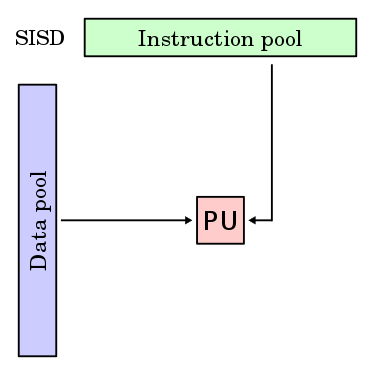
\includegraphics[width=0.3\linewidth]{./images/SISD.png} &
        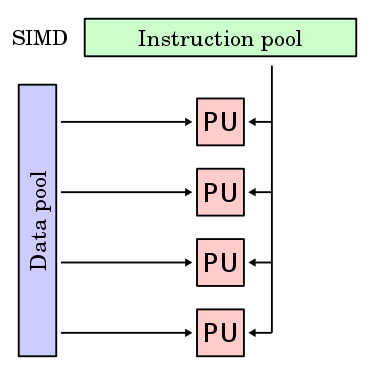
\includegraphics[width=0.3\linewidth]{./images/SIMD.png}   \\
        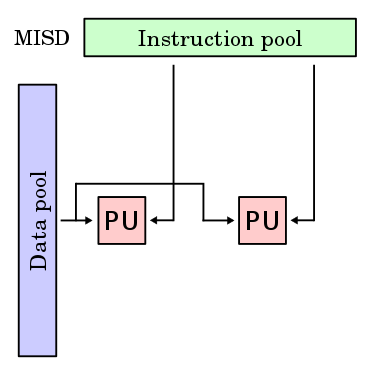
\includegraphics[width=0.3\linewidth]{./images/MISD.png} &
        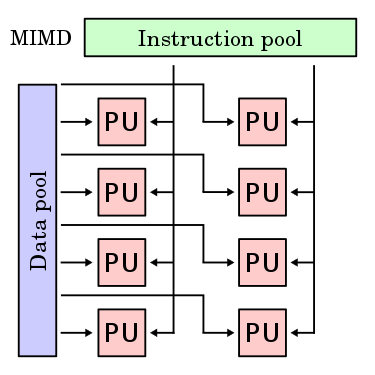
\includegraphics[width=0.3\linewidth]{./images/MIMD.png}   \\
    \end{tabular}
    \caption{Flynn's Taxonomy}
\end{figure}

\subsection{计算机系统结构定义}

\textbf{计算机系统结构}:机器语言程序员所看到的传统机器级所具有的\underline{属性}. 它确定计算机系统的软、硬件界面.

\textbf{计算机组成}:计算机系统结构的\underline{逻辑实现},包括五大功能部件组成以及逻辑设计等. 它着眼于机器级内\underline{各事件的排序方式与控制方式},各部件的功能以及各部件的联系.

\textbf{计算机实现}:计算机组成的\underline{物理实现},包括处理机、主存等部件的物理结构,器件的集成度和速度功耗,模块、插件、底板的划分与连接,信号传输,电源、冷却及整机装配技术等. 它着眼于器件技术和微组装技术,其中器件技术在实现技术中占主导作用.

计算机系统结构的现代定义:在满足功能、性能和价格目标的条件下,设计、选择和互连硬件部件构成计算机.

\textbf{指令集结构(ISA)}是硬件与软件之间的接口. 其特征有:

\begin{itemize}
    \item ISA 的类型:现代通用寄存器结构、早期累加器结构
    \item 存储器访问:按字节访问
    \item 寻址方式
    \item 操作数类型和大小:8 位字符、32 位整型数
    \item 操作类型:数据传输、算术/逻辑
    \item 控制流指令:转移、子程序调用/返回
    \item ISA 编码:固定长度、可变长度
\end{itemize}

\subsection{实现技术的趋势}

摩尔定律(Moore's Law):集成电路上可容纳的晶体管数目每隔两年就会增加一倍.

性能趋势:带宽改进优先于时延.

经验法则:成本减少速度与密度增加速度成比例,带宽增加速度与时延平方改进速度成比例.

\subsection{集成电路功耗的趋势}

经验法则:电压减少 $10\%$,功耗减少 $30\%$,性能减少 $<10\%$.

单核与双核:单核性能与面积增加倍数的一半成正比;多核有更高的功率利用率.

\subsection{可靠性}

提高可靠性的方法:冗余

\begin{itemize}
    \item 时间冗余:重复操作直到无错
    \item 资源冗余:配置另外的相同部件,有错时用于替代出错部件
\end{itemize}

\subsection{计算机主要性能指标}

响应时间(墙钟时间):从用户发出请求到得到响应的时间,包括等待 I/O 的时间. 是用户感觉到的系统速度.

CPU 时间:从程序开始执行到程序结束的时间,不包括等待 I/O 的时间. 测量设计者感觉到的 CPU 速度.

\begin{itemize}
    \item 用户 CPU 时间:花费在用户模式的时间
    \item 系统 CPU 时间:花费在内核模式的时间
\end{itemize}

吞吐量:单位时间内处理的任务数.

处理器用更快的型号替换可以改善响应时间和吞吐量;增加额外的处理器可以改善吞吐量.

工业性能指标 MIPS:每秒百万条指令.

总执行时间:$n$ 个测试程序的执行时间 $T$ 的算术平均值为 $\dfrac{1}{n}\sum\limits_{i=1}^{n}T_i$;如果性能用 Rate $R$(如 MIPS)表示, 那么总的执行时间平均值就是调和平均值 $\dfrac{n}{\sum\limits_{i=1}^{n}\dfrac{1}{R_i}}$.

通常,机器运行某些程序更频繁,则应该给这些程序更大的权值 $W$,算术平均值为 $\dfrac{1}{n}\sum\limits_{i=1}^{n}W_i \times T_i$;调和平均值为 $\dfrac{n}{\sum\limits_{i=1}^{n} \dfrac{W_i}{R_i}}$. 通常,$W_i$ 为程序的执行频率.

实用基准测试程序集 SPEC:以 CPU 时间为基准,以不同的工作负载为测试对象.

SPEC 率(SPEC Ratio)是一个测试程序在参考计算机上的执行时间与在被测计算机上的执行时间的比值,SPEC Ratio 越高,说明被测计算机的性能越好.

$$
    \text{SPEC Ratio} = \dfrac{t_{ref}}{t_{test}} = \dfrac{\text{参考计算机的执行时间}}{\text{被测计算机的执行时间}}
$$

被测试计算机的性能用执行 $n$ 个基准测试程序分别得到的 SPEC Ratio 的几何平均值来衡量(PPT 中表示为 SM):

$$
    \sqrt[n]{\prod\limits_{i=1}^{n} \text{SPEC Ratio}_i}
$$

\begin{table}[h]
    \centering
    \begin{tabular}{cccc}
        \hline
        \textbf{应用程序} & \textbf{Opteron SPEC Ratio} & \textbf{Itanium2 SPEC Ratio} & \textbf{Itanium/Opteron} \\
        \hline
        mesa          & 21.67                       & 12.99                        & 0.6                      \\
        applu         & 22.34                       & 41.25                        & 1.85                     \\
        lucas         & 22.52                       & 18.76                        & 0.83                     \\
        \dots         & \dots                       & \dots                        & \dots                    \\
        几何平均值         & 20.86                       & 27.12                        & 1.3                      \\
        \hline
    \end{tabular}
\end{table}

\begin{center}
    \fbox{
        \begin{minipage}{.95\linewidth}

            \textbf{例}:

            假如你的公司需要选购是 Opteron 还是 Itanium2. 公司的应用情况是:$50\%$ 的时间运行类似于 mesa 的应用程序,$25\%$ 的时间运行类似于 applu 应用程序,$25\%$ 的时间运行类似于 lucas 的应用程序. 上表提供了 Opteron 和 Itanium 的 SPEC Ratio 信息.

            (1)如果仅根据SPEC总体性能进行选择,你选择哪一种微处理器?为什么?

            (2)计算公司混合应用程序的 Itanium/Opteron SPEC Ratio 加权平均值是多少?按照这个结果应该选择哪一种微处理器?

            \textbf{解}:

            (1)

            选择 Itanium2,因为其几何平均值的值是 Opteron 的 1.3 倍,表明它的总的性能更好.

            (2)

            $0.6\times50\%+1.85\times25\%+0.83\times25\%=0.97$,表明针对公司的应用程序情况,选择 Opteron 有更好的性能.

        \end{minipage}
    }
\end{center}

\subsection{计算机设计的量化原则}

Amdahl 定律:采用更快的执行方式后所获得的系统性能提高,与这种执行方式的使用频率或占总执行时间的比例有关.

Amdahl 定律定义了一台计算机采用某种改进措施所取得的系统加速比:

$$
    \text{加速比} = \dfrac{\text{改进后的计算机性能}}{\text{改进后的计算机性能}} = \dfrac{\text{改进前的执行时间}}{\text{改进后的执行时间}}
$$

改进比例:

$$
    F_e = \dfrac{\text{改进部分的执行时间}}{\text{改进前的执行时间}}
$$

改进加速比:

$$
    S_e = \dfrac{\text{改进部分改进前的执行时间}}{\text{改进部分改进后的执行时间}}
$$

设改进后执行时间为 $T_e$,改进前的执行时间为 $T_0$,则:

$$
    T_e = T_0 \times (1 - F_e) + \dfrac{T_0 F_e}{S_e} = T_0 \left(1 - F_e + \dfrac{F_e}{S_e}\right)
$$

改进后整个系统的加速比为:

$$
    S_n = \dfrac{T_0}{T_e} = \dfrac{T_0}{T_0 \left(1 - F_e + \dfrac{F_e}{S_e}\right)} = \dfrac{1}{1 - F_e + \dfrac{F_e}{S_e}}
$$

提高改进比例 $F_e$ 或改进加速比 $S_e$ 可以提高系统加速比 $S_n$. 但是 $F_e$ 对 $S_n$ 的影响更大.

\begin{center}
    \fbox{
        \begin{minipage}{.95\linewidth}

            \textbf{例}:

            设一台计算机运行某程序的 CPU 时间如下:

            \begin{itemize}
                \item 浮点指令:60 s
                \item 整数指令:100 s
                \item 读写指令:40 s
                \item 分支指令:40 s
                \item 总时间:240 s
            \end{itemize}

            (1)如浮点指令执行时间减少50\%,总时间减少百分之多少?减少后加速比为多少?

            (2)如总时间减少15\%,只减少整数指令时间,整数指令时间减少百分之多少?

            (3)如只减少分支指令时间,总时间能否减少20\%?

            \textbf{解}:

            (1)

            浮点指令减少 50\% 时间:$60\times50\%= 30$ s

            总时间减少:$30/240 = 12.5\%$;

            加速比:$240/210 = 1.143$

            (2)

            总时间减少 15\% 时间:$240\times15\%= 36$ s

            减少的整数时间比例:$36/100=36\%$

            (3)

            不能,因为分支指令时间减少后,总时间减少的比例不够.

        \end{minipage}
    }
\end{center}

\section{指令系统原理与示例}

\subsection{指令集系统结构的分类}

不同指令集系统结构最根本的区别在于处理器内部数据的存储结构不同.

\textbf{存储结构}:堆栈、累加器或一组寄存器. 操作数可以显式指定或者隐含指定.

\begin{itemize}
    \item \textbf{堆栈结构}:操作数隐含地位于栈顶
    \item \textbf{累加器结构}:操作数隐含地位于累加器
    \item \textbf{通用寄存器结构}:只能明确地指定操作数(寄存器/存储器地址)
\end{itemize}

通用寄存器按照访问方式划分,主要有以下两种系统结构:

\begin{itemize}
    \item \textbf{寄存器-存储器结构}:一般指令都可以访问存储器
    \item \textbf{寄存器-寄存器结构}:只能通过 load 和 store 指令访问存储器
\end{itemize}

\subsection{存储器寻址}

\textbf{大小端模式}:存储器中的数据在存储器中的存放顺序.

\begin{itemize}
    \item \textbf{大端模式}:高位字节存放在低地址
    \item \textbf{小端模式}:低位字节存放在低地址
\end{itemize}

\textbf{地址对齐}:地址对齐是为了提高存储器的访问效率,使得存储器的访问速度与存储器的容量成正比.

假设一个 $s$ 字节数据的地址是 $A$,如果 $A$ 是 $s$ 的整数倍,那么这个数据就是地址对齐的.

\subsection{MIPS 指令集结构}

MIPS 系统结构是一种寄存器-存储器结构(load-store 结构),指令集结构是 RISC 结构.

\begin{itemize}
    \item 固定长度指令编码:32 位
    \item 32 个 64 位通用寄存器:R0-R31,其中 R0 的值永远是 0
    \item 32 个浮点寄存器:F0-F31
    \item 定点数据类型有 8 位字节、16 位半字、32 位字和 64 位双字
    \item 浮点数有 32 位单精度和 64 位双精度
\end{itemize}

MIPS 的指令格式:

\begin{itemize}
    \item I 类型:操作码(OP)+源寄存器(RS)+目的寄存器(RT)+立即数/偏移量(IMM)
    \item R 类型:操作码(OP)+源寄存器(RS)+源寄存器(RT)+目的寄存器(RD)+移位量(SHAMT)+功能码(FUNCT)
    \item J 类型:操作码(OP)+目的地址(ADDR)
\end{itemize}

MIPS 操作:载入和存储、ALU操作、分支与跳转、浮点操作.

\section{单周期 MIPS 处理器的设计}

\subsection{单周期实现}

单周期 CPU 设计:将每条指令的执行周期设为一个时钟周期,时钟周期需要满足所有指令的执行时间.

要实现的 MIPS 的指令子集(9 种):

\begin{itemize}
    \item R 型指令:\lstinline{add}、\lstinline{sub}、\lstinline{and}、\lstinline{or}、\lstinline{slt}、\lstinline{beq}
    \item I 型指令:\lstinline{lw}、\lstinline{sw}
    \item J 型指令:\lstinline{j}
\end{itemize}

以上指令集按功能可归纳为:

\begin{itemize}
    \item 存储器访问指令(I 型指令):\lstinline{lw}、\lstinline{sw}
    \item 算术逻辑指令(R 型指令):\lstinline{add}、\lstinline{sub}、\lstinline{and}、\lstinline{or}、\lstinline{slt}
    \item 分支指令(R 型指令):\lstinline{beq}
    \item 跳转指令(J 型指令):\lstinline{j}
\end{itemize}

使用该指令子集可以说明在建立数据通路和控制部件时的关键原理(该指令集没有包含乘、除和移位指令、浮点指令).

构建数据通路和控制部件:

\begin{figure}[h]
    \centering
    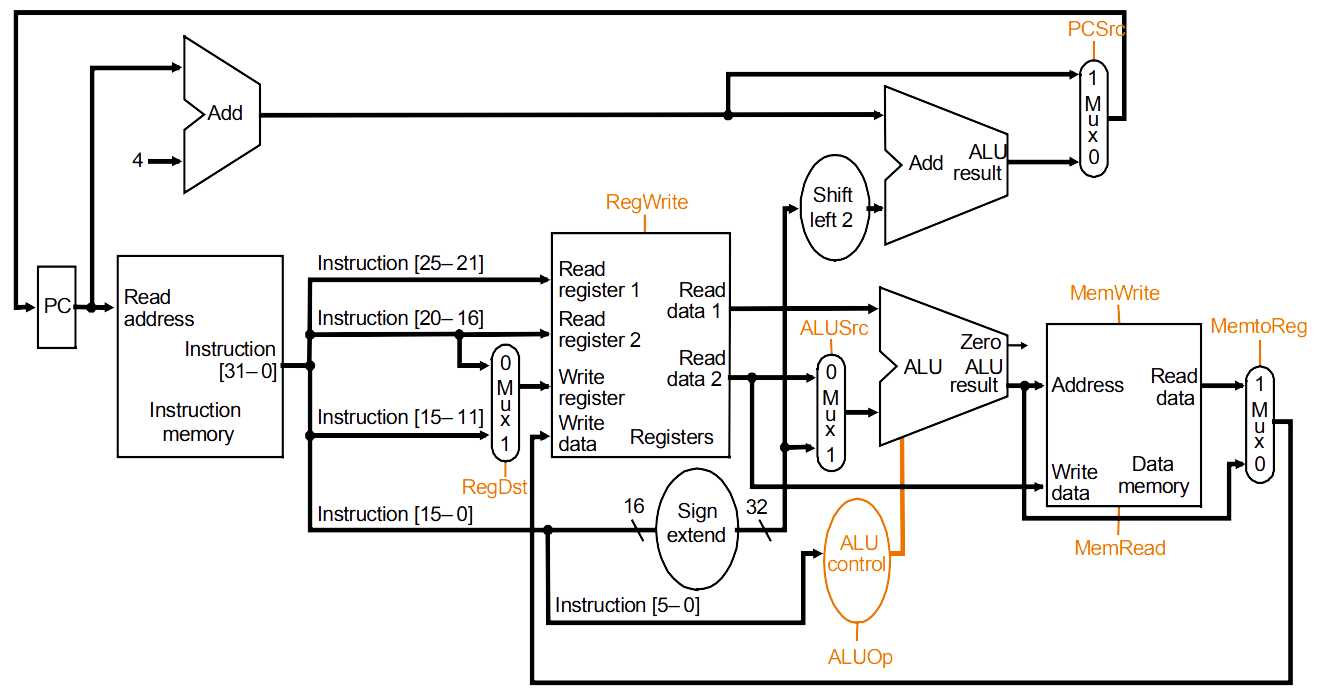
\includegraphics[width=\textwidth]{./images/Implementation.png}
\end{figure}

\subsection{数据通路}

R 型指令的数据通路:

\begin{figure}[h]
    \centering
    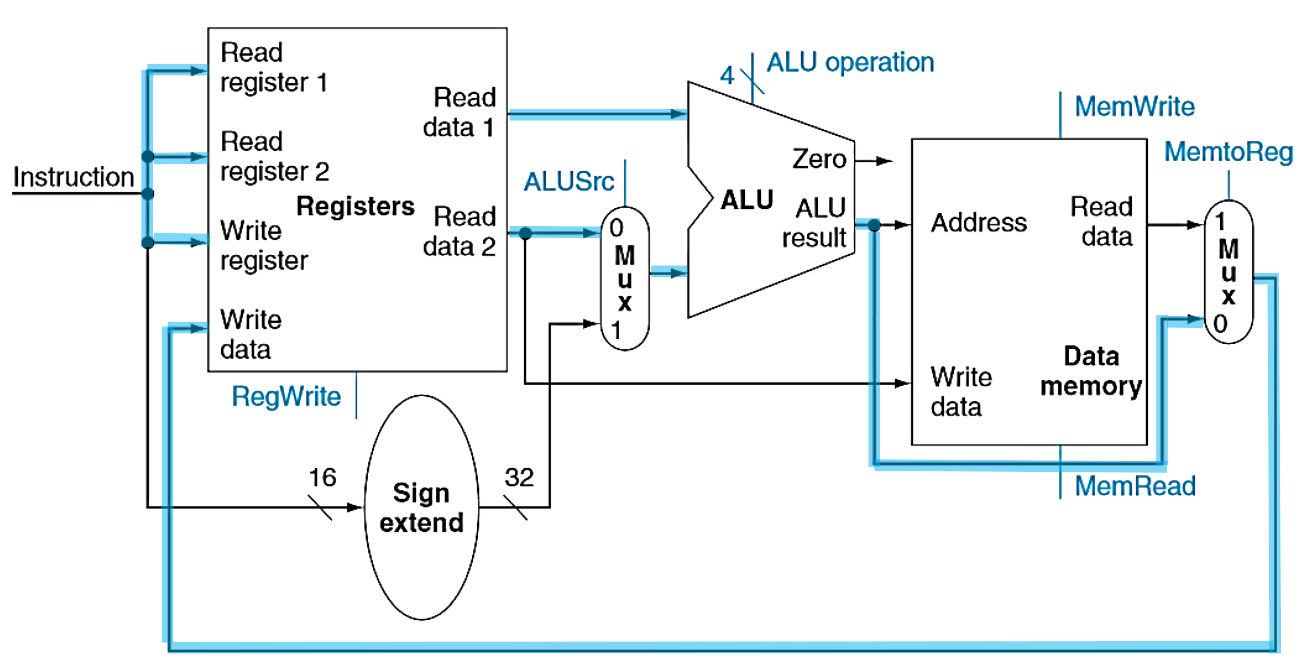
\includegraphics[width=0.7\textwidth]{./images/DATAPATH_R.png}
\end{figure}

\lstinline{lw} 指令的数据通路:

\begin{figure}[h]
    \centering
    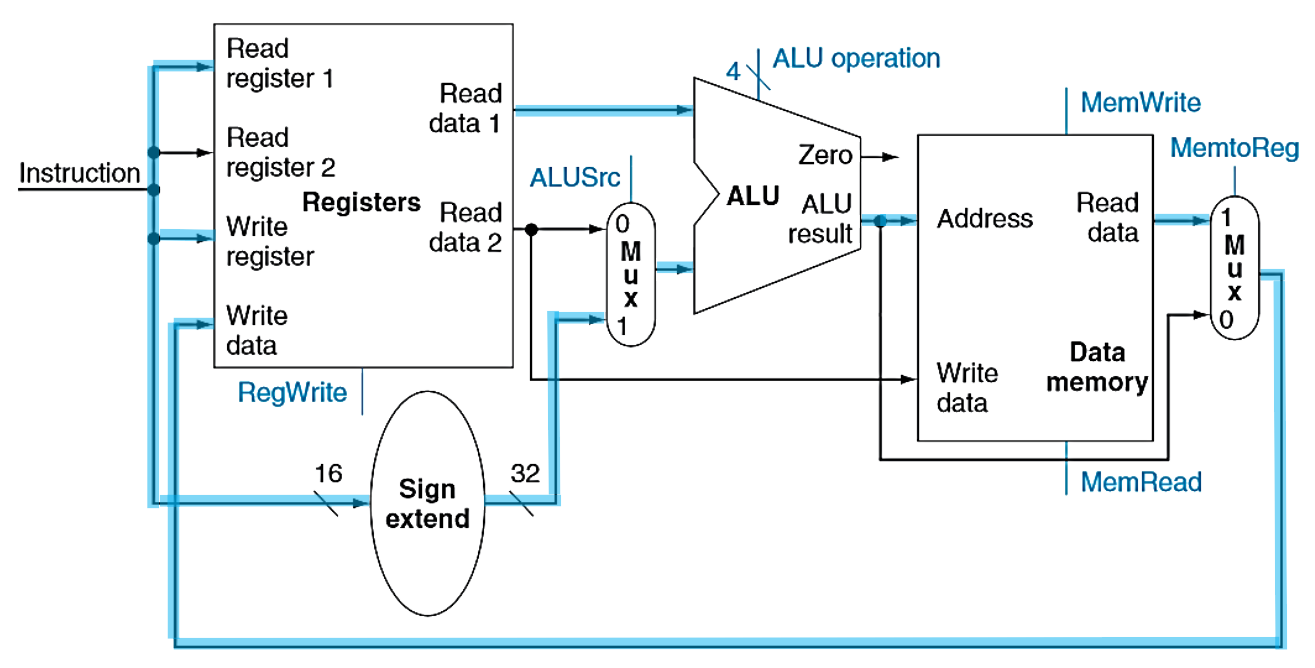
\includegraphics[width=0.7\textwidth]{./images/DATAPATH_LW.png}
\end{figure}

\lstinline{sw} 指令的数据通路:

\begin{figure}[h]
    \centering
    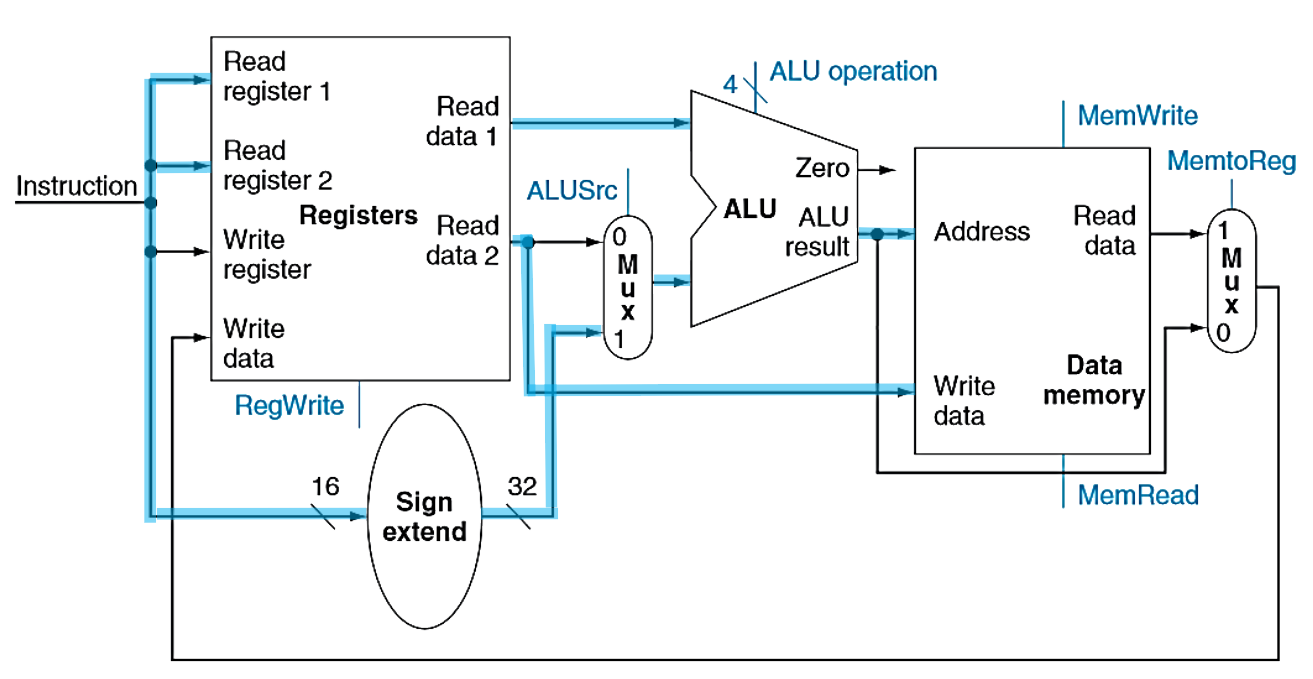
\includegraphics[width=0.7\textwidth]{./images/DATAPATH_SW.png}
\end{figure}

\lstinline{beq} 指令的数据通路:

\begin{figure}[h]
    \centering
    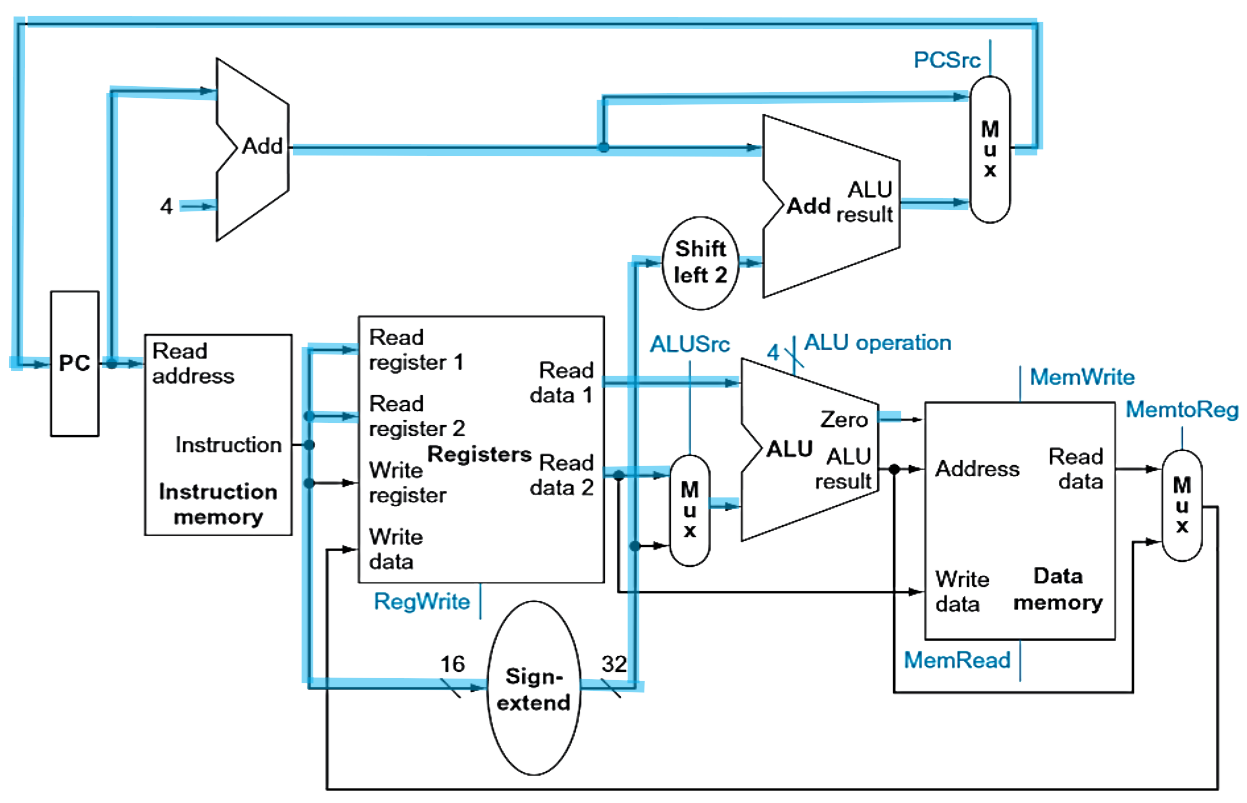
\includegraphics[width=0.7\textwidth]{./images/DATAPATH_BEQ.png}
\end{figure}

\subsection{控制信号}

各指令的控制信号:

\begin{table}[h]
    \centering
    \begin{tabular}{ccccccccc}
        \hline
            & RegDst & ALUSrc & Mem2Reg & RegWr & MemRd & MemWr & Branch & ALUOp \\
        \hline
        R   & 1      & 0      & 0       & 1     & 0     & 0     & 0      & 10    \\
        lw  & 0      & 1      & 1       & 1     & 1     & 0     & 0      & 00    \\
        sw  & X      & 1      & X       & 0     & 0     & 1     & 0      & 00    \\
        beq & X      & 0      & X       & 0     & 0     & 0     & 1      & 01    \\
        \hline
    \end{tabular}
\end{table}

有如下特征:

\begin{itemize}
    \item \lstinline{sw} 和 \lstinline{beq} 指令不写任何寄存器
    \item \lstinline{lw} 和 \lstinline{sw} 指令使用常数字段,它们还依赖 ALU 计算有效内存地址
    \item R 类型指令的 ALUOp 依赖于指令的 func 字段
    \item \lstinline{beq} 指令的 PCSrc 控制信号(未列出)为 1,ALU 有 Zero 输出
\end{itemize}

\section{流水线技术及指令级并行}

\subsection{流水线的概念}

流水线技术:将指令的执行周期分为多个时钟周期,每个时钟周期执行一部分指令.

流水线的分类:

\begin{itemize}
    \item 按功能分类:单功能流水线、多功能流水线
    \item 按工作方式分类:静态流水线、动态流水线
\end{itemize}

\subsection{流水线的时空图及性能分析}

时空图:时空图从时间和空间两个方面描述了流水线的工作过程. 时空图中,横坐标代表时间,纵坐标代表流水线的各个段(或级,即完成一条指令的一部分操作).

吞吐率:在单位时间内流水线所完成的任务数量或输出结果的数量.

$$
    \text{TP} = \frac{n}{T}
$$

各段时间均相等的 $k$ 段线性流水线的实际吞吐率:

$$
    \text{TP} = \frac{n}{T} = \frac{n}{(k+n-1)\Delta t}
$$

最大吞吐率:

$$
    \text{TP}_\text{max} = \frac{1}{\Delta t}
$$

各段时间不完全相等的流水线的最大吞吐率:

$$
    \text{TP}_\text{max} = \frac{1}{\max(\Delta t_i)}
$$

解决流水线瓶颈问题的常用方法:细分瓶颈段、重复设置瓶颈段.

衡量流水线性能的主要指标有:吞吐率、加速比、效率.

多功能流水线的时空图:静态/动态.

\begin{center}
    \fbox{
        \begin{minipage}{.95\linewidth}

            \textbf{例}:

            计算 $\sum\limits_{i=1}^4 a_i b_i$,画出下图所示多功能流水线在静态和动态下的时空图,并分析其性能.

            \begin{minipage}{.9\linewidth}
                \centering
                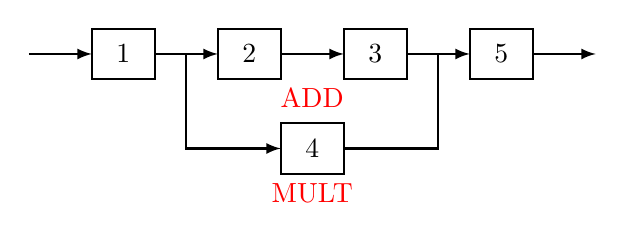
\begin{tikzpicture}[thick,scale=.8]
                    \foreach \i in {0,2,4,6} {
                            \draw (\i,5.1) rectangle (\i+1,5.9);
                        }

                    \draw (3,3.6) rectangle (4,4.4);

                    \node at (0.5,5.5) {$1$};
                    \node at (2.5,5.5) {$2$};
                    \node at (4.5,5.5) {$3$};
                    \node at (3.5,4) {$4$};
                    \node at (6.5,5.5) {$5$};

                    \draw[color=red] node at (3.5,4.8) {ADD};
                    \draw[color=red] node at (3.5,3.3) {MULT};

                    \draw[-latex] (-1,5.5) -- (0,5.5);
                    \draw[-latex] (1,5.5) -- (2,5.5);
                    \draw[-latex] (3,5.5) -- (4,5.5);
                    \draw[-latex] (5,5.5) -- (6,5.5);
                    \draw[-latex] (7,5.5) -- (8,5.5);

                    \draw[-latex] (1.5,5.5) -- (1.5,4) -- (3,4);
                    \draw (4,4) -- (5.5,4) -- (5.5,5.5);

                \end{tikzpicture}
            \end{minipage}

            \textbf{解}:

            计算过程分解为 4 次乘法和 3 次加法:

            $$
                \begin{aligned}
                    \text{①} & \text{MUL}_1: a_1 \times b_1              \\
                    \text{②} & \text{MUL}_2: a_2 \times b_2              \\
                    \text{③} & \text{MUL}_3: a_3 \times b_3              \\
                    \text{④} & \text{MUL}_4: a_4 \times b_4              \\
                    \text{⑤} & \text{ADD}_1: \text{MUL}_1 + \text{MUL}_2 \\
                    \text{⑥} & \text{ADD}_2: \text{MUL}_3 + \text{MUL}_4 \\
                    \text{⑦} & \text{ADD}_3: \text{ADD}_1 + \text{ADD}_2
                \end{aligned}
            $$

            静态流水线时空图如下:

            \begin{minipage}{.9\linewidth}
                \centering
                \begin{tikzpicture}[thick,scale=.8]
                    \foreach \i in {0,1,...,5}{
                            \foreach \j in {0,1,...,14} {
                                    \draw (\j+0.5,\i+0.5) -- (\j+1.5,\i+0.5);
                                }
                        }
                    \foreach \i in {0,1,...,15}{
                            \foreach \j in {0,1,...,4} {
                                    \draw (\i+0.5,\j+0.5) -- (\i+0.5,\j+1.5);
                                }
                        }
                    \foreach \i in {1,...,5}{
                            \node[left] at (0.5,\i) {$\i$};
                        }
                    \foreach \i in {0,...,15}{
                            \node[below] at (\i+0.5,0.5) {$\i$};
                        }

                    \node at (1,1) {①};
                    \node at (2,4) {①};
                    \node at (3,5) {①};

                    \node at (2,1) {②};
                    \node at (3,4) {②};
                    \node at (4,5) {②};

                    \node at (3,1) {③};
                    \node at (4,4) {③};
                    \node at (5,5) {③};

                    \node at (4,1) {④};
                    \node at (5,4) {④};
                    \node at (6,5) {④};

                    \node at (7,1) {⑤};
                    \node at (8,2) {⑤};
                    \node at (9,3) {⑤};
                    \node at (10,5) {⑤};

                    \node at (8,1) {⑥};
                    \node at (9,2) {⑥};
                    \node at (10,3) {⑥};
                    \node at (11,5) {⑥};

                    \node at (12,1) {⑦};
                    \node at (13,2) {⑦};
                    \node at (14,3) {⑦};
                    \node at (15,5) {⑦};
                \end{tikzpicture}
            \end{minipage}

            吞吐率 $\text{TP} = \dfrac{7}{15\Delta T}$;效率 $\text{EFF} = \dfrac{3 \times 4 + 4 \times 3}{5 \times 15}$;加速比 $\text{SP} = \dfrac{7 \times 5}{15}$.

            动态流水线时空图如下:

            \begin{minipage}{.9\linewidth}
                \centering
                \begin{tikzpicture}[thick,scale=.8]
                    \foreach \i in {0,1,...,5}{
                            \foreach \j in {0,1,...,14} {
                                    \draw (\j+0.5,\i+0.5) -- (\j+1.5,\i+0.5);
                                }
                        }
                    \foreach \i in {0,1,...,15}{
                            \foreach \j in {0,1,...,4} {
                                    \draw (\i+0.5,\j+0.5) -- (\i+0.5,\j+1.5);
                                }
                        }
                    \foreach \i in {1,...,5}{
                            \node[left] at (0.5,\i) {$\i$};
                        }
                    \foreach \i in {0,...,15}{
                            \node[below] at (\i+0.5,0.5) {$\i$};
                        }

                    \node at (1,1) {①};
                    \node at (2,4) {①};
                    \node at (3,5) {①};

                    \node at (2,1) {②};
                    \node at (3,4) {②};
                    \node at (4,5) {②};

                    \node at (3,1) {③};
                    \node at (4,4) {③};
                    \node at (5,5) {③};

                    \node at (4,1) {④};
                    \node at (5,4) {④};
                    \node at (6,5) {④};

                    \node at (5,1) {⑤};
                    \node at (6,2) {⑤};
                    \node at (7,3) {⑤};
                    \node at (8,5) {⑤};

                    \node at (7,1) {⑥};
                    \node at (8,2) {⑥};
                    \node at (9,3) {⑥};
                    \node at (10,5) {⑥};

                    \node at (11,1) {⑦};
                    \node at (12,2) {⑦};
                    \node at (13,3) {⑦};
                    \node at (14,5) {⑦};
                \end{tikzpicture}
            \end{minipage}

            吞吐率 $\text{TP} = \dfrac{7}{14\Delta T}$;效率 $\text{EFF} = \dfrac{3 \times 4 + 4 \times 3}{5 \times 14}$;加速比 $\text{SP} = \dfrac{7 \times 5}{14}$.

        \end{minipage}
    }
\end{center}

\subsection{流水线中的冒险问题}

\textbf{数据冒险(Data Hazard)}:指令的操作数尚未准备好,而该指令已经进入流水线的下一阶段而导致的冒险.

\textbf{结构冒险(Structural Hazard)}:某些指令组合在流水线中重叠执行时产生了资源冲突而导致的冒险.

\textbf{控制冒险(Control Hazard)}:因为程序的执行方向可能被改变而存在的冒险.

\textbf{数据冒险的解决}:

数据前推:将数据从流水线的前一阶段传递到后一阶段. \lstinline{lw} 数据冒险需要额外的暂停周期.

\begin{figure}[h]
    \centering
    \begin{tikzpicture}[thick,scale=.75]
        \foreach \i in {0,1,...,8}{
                \draw[-latex] (2*\i,11.5) -- (2*\i,12);
                \draw (2*\i,12) -- (2*\i+1,12);
                \draw[-latex] (2*\i+1,12) -- (2*\i+1,11.5);
                \draw (2*\i+1,11.5) -- (2*\i+2,11.5);
            }

        \draw[-latex] (18,11.5) -- (18,12);

        \draw (0,10) rectangle node {\lstinline{lw}} (2,11);
        \draw (2,10) rectangle node {\lstinline{$1,33}} (4,11);
        \draw (4,10) rectangle node {} (6,11);
        \draw (6,10) rectangle node {\textcolor{blue}{MEM}} (8,11);
        \draw (8,10) rectangle node {\textcolor{red}{\lstinline{$3}}} (10,11);

        \draw (2,8) rectangle node {\lstinline{or}} (4,9);
        \draw (4,8) rectangle node {\text{STALL}} (6,9);
        \draw (6,8) rectangle node {\lstinline{$9,}\textcolor{red}{\lstinline{$3}}} (8,9);
        \draw (8,8) rectangle node {} (10,9);
        \draw (10,8) rectangle node {} (12,9);
        \draw (12,8) rectangle node {\lstinline{$2}} (14,9);

        \draw (6,6) rectangle node {\lstinline{add}} (8,7);
        \draw (8,6) rectangle node {\lstinline{$3,$10}} (10,7);
        \draw (10,6) rectangle node {\textcolor{blue}{EX}} (12,7);
        \draw (12,6) rectangle node {} (14,7);
        \draw (14,6) rectangle node {\textcolor{red}{\lstinline{$5}}} (16,7);

        \draw (8,4) rectangle node {\lstinline{sub}} (10,5);
        \draw (10,4) rectangle node {\textcolor{red}{\lstinline{$5}}\lstinline{,$4}} (12,5);
        \draw (12,4) rectangle node {} (14,5);
        \draw (14,4) rectangle node {} (16,5);
        \draw (16,4) rectangle node {\lstinline{$6}} (18,5);

        \draw[-latex,red] (8.2,10.5) -- (8.2,8.5);
        \draw[-latex,red] (12.2,6.5) -- (12.2,4.5);
    \end{tikzpicture}
\end{figure}

\textbf{控制冒险的解决}:提前计算分支目标地址、提前判断分支条件,以及提前预测分支的执行方向.

在 ID 级中已形成了PC值和地址偏移量,因此将分支地址计算从 EX 级前移到 ID 级即可. 分支预测错误的代价减小到 1 条指令.

\begin{itemize}
    \item R 型指令 + \lstinline{beq} 指令:需暂停 1 个时钟周期
    \item \lstinline{lw} + \lstinline{beq} 指令:需暂停 2 个时钟周期
\end{itemize}

分支指令 \lstinline{beq} 与其前面 R 型指令的数据冒险处理:

\begin{itemize}
    \item 无数据冒险时:IF.Flush 冲掉 IF/ID 寄存器,预取到的指令变成 \lstinline{nop}
    \item 有数据冒险时:保持 PC 和 IF/ID 不变,指令编码不变,并将该指令的所有写信号全部关闭
\end{itemize}

\subsection{流水线中异常的处理}

停止和重新开始执行的步骤:

\begin{itemize}
    \item 强制一个 \lstinline{trap} 指令进入流水线
    \item 关掉出错指令及后面指令的所有写操作,直到 \lstinline{trap} 指令开始执行
    \item 当 \lstinline{trap} 指令开始执行,唤醒 OS ,OS 保存出错指令的 PC 值
    \item OS 试图修复异常,然后重新执行出错指令
\end{itemize}

异常在 MIPS 体系结构中的处理:

\begin{itemize}
    \item 异常发生时:在异常程序计数器(EPC)中保存出错指令的地址,并把控制权转交给 OS
    \item 在完成处理异常所需动作后,OS 可以终止程序,也可以继续执行程序,此时由 EPC 决定重新开始执行的地方
\end{itemize}

\subsection{动态调度算法}

见记分牌算法与 Tomasulo 算法专题.

\section{存储系统}

\subsection{存储器}

\textbf{存储器的分类与参数}:

\begin{itemize}
    \item 半导体存储器:容量、存储周期
          \begin{itemize}
              \item 静态随机存储器(SRAM)
              \item 动态随机存储器(DRAM)
              \item 闪存(Flash Memory)
          \end{itemize}
    \item 磁表面存储器:容量、转速
    \item 光盘存储器
          \begin{itemize}
              \item 只读性光盘(CD-ROM)
              \item 写入式光盘(WORM)
              \item 可擦写光盘(CD-RW)
          \end{itemize}
\end{itemize}

\textbf{存储器的存取方式}:

\begin{itemize}
    \item 随机存取存储器(RAM)
    \item 顺序存取存储器(SAM)
\end{itemize}

\textbf{存储器的主要性能指标}:

\begin{itemize}
    \item 存储容量
    \item 存取周期
\end{itemize}

\subsection{Cache 基本原理}

Cache 是按\textbf{块(block)}进行管理的. Cache 和主存均被分割成大小相同的块. 对 Cache 和主存的访问是以块为基本单位.

\subsubsection{映像规则}

\textbf{直接映像}:块只能放在 Cache 中唯一的位置.

\textbf{全相联}:块可以放在 Cache 中的任意位置.

\textbf{组相联}:块能够放在 Cache 一组中任意一块位置. 如果一组有 $n$ 块,则称为 $n$ 路组相联.

\subsubsection{块的识别}

物理地址的格式:\textbf{标识 Tag} + \textbf{索引 Index} + \textbf{字节位移量 Byte Offset}.

\textbf{标识 Tag}:用于查找在 Cache 或一组中的匹配块.

\textbf{索引 Index}:选择块(直接映像 Cache)或组(组相联 Cache). 位数是 $\log_2(\text{块数/组数})$.

\textbf{字节位移量 Byte Offset}:选择块中的某个字节. 位数是 $\log_2(\text{块字节数})$.

\begin{center}
    \fbox{
        \begin{minipage}{.95\linewidth}

            \textbf{例}:

            数据 Cache 容量为 16KB,块大小为 32B,最小寻址单位 1 字节,采用两路组相联映像方式, Cache 的物理地址为 36 位. 计算索引、标识、块内偏移量的位数.

            \textbf{解}:

            块内偏移:$32=2^5$,占 5 位(低 5 位).

            索引: $\dfrac{\text{Cache 容量}}{\text{组数} \times \text{块大小}} = \dfrac{16 \times 1024}{2 \times 32} = 2^8$,占 8 位(中间 8 位).

            标识:$36 - 8 - 5 = 23$,占 23 位(高23位).

        \end{minipage}
    }
\end{center}

\subsubsection{块的替换策略}

\textbf{随机替换}:
\begin{itemize}
    \item 随机选择一组中的一块作为被替换块
    \item 硬件容易实现,需要随机数产生器
    \item 均匀使用一组中的各块
    \item 可能替换即将被访问的那一块
\end{itemize}

\textbf{最近最少使用(LRU)}:
\begin{itemize}
    \item 选择一组中最近最少被访问的块作为被替换块
    \item 假定最近被访问的块很可能会一再访问
    \item 需要额外的位记录访问历史
\end{itemize}

\textbf{先进先出(FIFO)}:
\begin{itemize}
    \item 选择一组中最先进入 Cache 的一块
\end{itemize}

\begin{center}
    \fbox{
        \begin{minipage}{.95\linewidth}

            \textbf{例}:

            Cache-主存存储层次中,主存有 0-15 共 16 块,Cache 为 8 块,块号为 C0-C7,采用 2 路组相联映像. 设 Cache 初始为空,现访存块地址流为 $1, 1, 2, 4, 13, 3, 9, 7, 3, 13$ 时:

            (1)分别画出用 LRU 替换算法和 FIFO 替换算法,Cache 内各块的实际替换过程图,并标出命中时刻.

            (2)计算命中率.

            \textbf{解}:

            (1)见下页表

            (2)$3/10=0.3$,$3/10=0.3$.

        \end{minipage}
    }
\end{center}

\begin{table}[h]
    \centering
    \begin{tabular}{ccccccccccc}
        \hline
        \multirow{2}{*}{Cache 块} & \multicolumn{10}{c}{主存块地址流}                                                 \\
        \cline{2-11}
                                 & 1                           & 1  & 2  & 4  & 13 & 3  & 9   & 7   & 3   & 13 \\
        \hline
        C0                       &                             &    &    & 4* & 4* & 4* & 4*  & 4*  & 4*  & 4* \\
        C1                       &                             &    &    &    &    &    &     &     &     &    \\
        C2                       & 1*                          & 1* & 1* & 1* & 1* & 1* & 9   & 9   & 9   & 9* \\
        C3                       &                             &    &    &    & 13 & 13 & 13* & 13* & 13* & 13 \\
        C4                       &                             &    & 2* & 2* & 2* & 2* & 2*  & 2*  & 2*  & 2* \\
        C5                       &                             &    &    &    &    &    &     &     &     &    \\
        C6                       &                             &    &    &    &    & 3* & 3*  & 3*  & 3   & 3  \\
        C7                       &                             &    &    &    &    &    &     & 7   & 7*  & 7* \\
        \hline
        命中                       &                             & H  &    &    &    &    &     &     & H   & H  \\
        \hline
    \end{tabular}
\end{table}

\begin{table}[h]
    \centering
    \begin{tabular}{ccccccccccc}
        \hline
        \multirow{2}{*}{Cache 块} & \multicolumn{10}{c}{主存块地址流}                                                  \\ \cline{2-11}
                                 & 1                           & 1  & 2  & 4  & 13 & 3  & 9   & 7   & 3   & 13  \\ \hline
        C0                       &                             &    &    & 4* & 4* & 4* & 4*  & 4*  & 4*  & 4*  \\
        C1                       &                             &    &    &    &    &    &     &     &     &     \\
        C2                       & 1*                          & 1* & 1* & 1* & 1* & 1* & 9   & 9   & 9   & 9   \\
        C3                       &                             &    &    &    & 13 & 13 & 13* & 13* & 13* & 13* \\
        C4                       &                             &    & 2* & 2* & 2* & 2* & 2*  & 2*  & 2*  & 2*  \\
        C5                       &                             &    &    &    &    &    &     &     &     &     \\
        C6                       &                             &    &    &    &    & 3* & 3*  & 3*  & 3*  & 3*  \\
        C7                       &                             &    &    &    &    &    &     & 7   & 7   & 7   \\
        命中                       &                             & H  &    &    &    &    &     &     & H   & H   \\ \hline
    \end{tabular}
\end{table}

\subsubsection{块的写策略}

\textbf{写直达策略}:写 Cache 的同时也写主存,读缺失不会导致替换时的写操作,保持了数据一致性,实现简单.
\begin{itemize}
    \item Cache 中的数据可以随时丢弃
    \item 只需要 valid 控制位
    \item 主存(或其他处理器)总是有最新的数据
\end{itemize}

\textbf{写回策略}:写 Cache 时不写主存,速度更快,主存带宽更低.
\begin{itemize}
    \item 不能丢弃 Cache 中的数据
    \item 需要 valid 位和 dirty 位
    \item 对同一块的多次写仅需要对主存写一次
\end{itemize}


\textbf{按写分配}:
\begin{itemize}
    \item 写失效时,把所写单元所在的块调入 Cache,然后再进行写命中操作
    \item 与读失效类似
    \item 写回 Cache 通常采用
\end{itemize}

\textbf{不按写分配}:
\begin{itemize}
    \item 写失效时,直接将值写入下一级存储器而不将相应的块调入 Cache
    \item 写的值不在 Cache 中
    \item 写直达 Cache 通常采用
\end{itemize}


\begin{center}
    \fbox{
        \begin{minipage}{.95\linewidth}

            \textbf{例}:

            假设有一个全相联映射有多个项的 Cache,采用写回策略,刚开始时 Cache 为空. 有下面 5 个存储器操作:

            \parindent=2em

            \lstinline{write Mem[100];}\par
            \lstinline{write Mem[100];}\par
            \lstinline{read  Mem[200];}\par
            \lstinline{write Mem[200];}\par
            \lstinline{write Mem[100];}

            \parindent=0em

            分别求按写分配和不按写分配情况下的命中次数和缺失次数.

            \textbf{解}:

            按写分配:

            \begin{itemize}
                \item \lstinline{write Mem[100];}:Cache 缺失,调入 Cache.
                \item \lstinline{write Mem[100];}:Cache 命中.
                \item \lstinline{read  Mem[200];}:Cache 缺失,调入 Cache.
                \item \lstinline{write Mem[200];}:Cache 命中.
                \item \lstinline{write Mem[100];}:Cache 命中.
            \end{itemize}

            不按写分配:

            \begin{itemize}
                \item \lstinline{write Mem[100];}:Cache 缺失.
                \item \lstinline{write Mem[100];}:Cache 缺失.
                \item \lstinline{read  Mem[200];}:Cache 缺失,调入 Cache.
                \item \lstinline{write Mem[200];}:Cache 命中.
                \item \lstinline{write Mem[100];}:Cache 缺失.
            \end{itemize}

        \end{minipage}
    }
\end{center}

\subsection{Cache 的性能分析}

\subsubsection{Cache 的命中率}

\textbf{平均访存时间}:

$$
    \begin{aligned}[b]
        \mathrm{AMAT} & = \text{命中时间} + \text{失效率} \times \text{失效开销}                                                  \\
                      & = \text{访问指令所占的百分比} \times \left(\text{指令命中时间} + \text{指令失效率} \times \text{失效开销} \right)       \\
                      & \quad + \text{访问数据所占的百分比} \times \left(\text{数据命中时间} + \text{数据失效率} \times \text{失效开销} \right)
    \end{aligned}
$$

\begin{center}
    \fbox{
        \begin{minipage}{.95\linewidth}

            \textbf{例}:

            假设 Cache 的命中时间为一个时钟周期,失效开销为 50 个时钟周期,在混合 Cache 中一次 LOAD 或 STORE 操作访问 Cache 的命中时间都要增加一个时钟周期. 又假设采用写直达策略,且有一个写缓冲器,并且忽略写缓冲器引起的等待. 约 75\% 的访存为取指令,则剩下 25\% 的访存是取数据. 请问指令 Cache 和数据 Cache 容量均为 16 KB 的分离 Cache 和容量为 32 KB 的混合 Cache 的平均访存时间各是多少?

            \textbf{解}:

            $$
                \begin{aligned}
                    \text{平均访存时间}_\text{分离} & = 75 \% \times(1+0.64 \% \times 50) + 25 \% \times(1 + 6.47 \% \times 50)      \\
                                            & = (75 \% \times 1.32) + (25 \% \times 4.325) = 0.990 + 1.059 = 2.05            \\
                    \text{平均访存时间}_\text{混合} & = 75 \% \times(1+1.99 \% \times 50) + 25 \% \times (1 + 1 + 1.99 \% \times 50) \\
                                            & = (75 \% \times 1.995) + (25 \% \times 2.995) = 1.496 + 0.749 = 2.24
                \end{aligned}
            $$

        \end{minipage}
    }
\end{center}

\textbf{CPU 执行时间}:

$$
    \notag
    \begin{aligned}[b]
        \mathrm{CPU \text{时间}} & = \text{IC} \times \left(\text{CPI}_\text{EX} + \dfrac{\text{访存次数}}{\text{指令数}} \times \text{失效率} \times \text{失效开销周期} \right) \times \text{时钟周期} \\& = \text{IC} \times \left(\text{CPI}_\text{EX} \times \text{时钟周期} + \dfrac{\text{访存次数}}{\text{指令数}} \times \text{失效率} \times \text{失效开销时间} \right) \\
    \end{aligned}
$$

\begin{center}
    \fbox{
        \begin{minipage}{.95\linewidth}

            \textbf{例}:

            给定以下的假设,试计算直接映象 Cache 和两路组相联 Cache 的平均访问时间以及 CPU 的性能.

            (1)理想 Cache 情况下的 CPI 为 2.0,时钟周期为 2 ns,平均每条指令访存 1.2 次.

            (2)两者 Cache 容量均为 64KB,块大小都是 32B.

            (3)两路组相联 Cache 中的多路选择器使 CPU 的时钟周期增加了 12\%.

            (4)这两种 Cache 的失效开销都是 80 ns.

            (5)命中时间为 1 个时钟周期.

            (6)直接映象 Cache 的失效率为 1.4\%,两路组相联 Cache 的失效率为 1.0\%.

            \textbf{解}:

            $$
                \begin{aligned}
                    \text{平均访存时间}_\text{直接}    & = 2 + 1.4\% \times 80 = 3.12                    \\
                    \text{平均访存时间}_\text{两路组相联} & = 2 \times (1 + 12\%)  + 1.0\% \times 80 = 3.04
                \end{aligned}
            $$
            $$
                \begin{aligned}
                    \mathrm{CPU \text{时间}}_\text{直接}    & = \text{IC} \times \left(2.0 \times 2 + 1.2 \times 1.4\% \times 80 \right)= 5.344 \text{IC}                   \\
                    \mathrm{CPU \text{时间}}_\text{两路组相联} & = \text{IC} \times \left(2.0 \times 2 \times (1 + 12\%) + 1.2 \times 1.0\% \times 80 \right) = 5.44 \text{IC}
                \end{aligned}
            $$

        \end{minipage}
    }
\end{center}

\subsection{降低 Cache 缺失率}

Cache 失效分为 3 类:强制性失效、容量失效、冲突失效.

\begin{itemize}
    \item 减少冲突失效,可以增加组的数目,全相联不会发生冲突失效
    \item 减小容量失效,可以增大 Cache 的容量
    \item 减少强制性失效,可以增大 Cache 块的容量
\end{itemize}

许多降低失效率的方法会增加命中时间或失效开销,降低失效率的方法:

\begin{itemize}
    \item 增大 Cache 块容量:减少了强制性失效,但增加了容量失效
    \item 提高相联度:减少了冲突失效,但增加了命中时间
    \item 增大 Cache 容量:减少了容量失效和冲突失效
    \item 编译器优化:合并数组、循环交换、循环融合
\end{itemize}

减小 Cache 失效开销:采用两级 Cache、关键字优先和提前重启动、让读失效优先于写、牺牲缓存、非阻塞 Cache、预取技术.

\subsection{快表 TLB}

虚拟地址到物理地址的转换需要 2 次访存,一次是访问页表取得物理地址,一次是访问物理内存取得数据.

快表 TLB 是一种高速缓存,用于存储虚拟地址到物理地址的映射.

快表 TLB 的缺失:TLB 中没有一个表项能匹配虚拟地址.

\begin{itemize}
    \item 页在主存中,只需要创建缺失的表项
    \item 页不在主存中,需要将控制权交给操作系统来处理
\end{itemize}

当处理缺失时,需要查找页表项,如果匹配的页表项的有效位无效,则该页就不在主存中. 如果有效位有效,则取回所需的表项.

访存时间:

\begin{itemize}
    \item 最好情况:虚拟地址由 TLB 转换,然后送到 Cache,找到相应的数据,然后取回并送入处理器
    \item 最坏情况:TLB、页表、Cache 三个部件都发生缺失
\end{itemize}

\end{document}
